\chapter{Θεωρητικό και Τεχνολογικό υπόβαθρο}
\label{chap3}

Σε αυτό το κεφάλαιο θα γίνει μια εκτεταμένη ανάλυση όλων των βασικών εννοιών που θεμελιώνουν τόσο τη θεωρητική, όσο και την τεχνολογική βάση στην οποία στηρίζεται η διπλωματική εργασία. Καθώς το παρόν έργο αποτελεί συγκερασμό δύο επιστημονικών κλάδων (Κοινωνιολογία και Πληροφορική), είναι αναγκαία η διαίρεση αυτού του κεφαλαίου σε ΠΟΣΕΣ ενότητες. Στην ενότητα 3.1 αναλύεται το θεωρητικό μοντέλο και οι κοινωνιολογικές έννοιες που το συνιστούν. Η ενότητα 3.2 αναφέρεται σε σχετικές ερευνητικές προσπάθειες που έχουν προηγηθεί. Τέλος, στην ενότητα 3.3 παρατίθενται τα σχετικά τεχνολογικά εργαλεία που χρησιμοποιήθηκαν.

\section{Θεωρητικό Υπόβαθρο - Βασικές Έννοιες}

\subsection{Κοινωνικός Ρόλος των Σύγχρονων Εφαρμογών}
Πρωταρχικό ρόλο στην επιτυχία μιας εφαρμογής παίζει το κίνητρο με το οποίο αυτή εξαφαλίζει τη διαρκή ενασχόληση του χρήστη. Βασικό στοιχείο για να επιτευχθεί αυτό είναι o κοινωνικός ρόλος που επωμίζεται ο χρήστης εντός της εφαρμογής. Oι σημερινές εφαρμογές έχουν στρέψει την προσοχή γύρω από την κοινωνική προβολή και επιβολή, απομακρύνοντας την προσοχή από δημοσιεύσεις που αφορούν κοινωνικά δρώμενα, τεχνολογικά επιτεύγματα και γενικότερα τον συλλογικό βίο (βλ. Σχ. \ref{socialsharing}). Έτσι, παρατηρείται η προσκόλληση στα μέσα κοινωνικής δικτύωσης ως τρόπο άσκησης κοινωνικής επιρροής. Δημιουργούνται συνεπώς εγωκεντρικές τάσεις που τροφοδοτούν νέες ανάγκες και οδηγούν σε νέες ομοειδείς εφαρμογές. Τέτοια παραγείγματα είναι η ανάγκη για δημοτικότητα και κοινωνική αποδοχή \cite{[IND+16]} από τρίτους, η έντονη εμμονή με την προσωπική εικόνα στον ψηφιακό κόσμο και η ενίσχυση των απρόσωπων σχέσεων \cite{[JAR+18]}. 

\begin{figure}[H]
    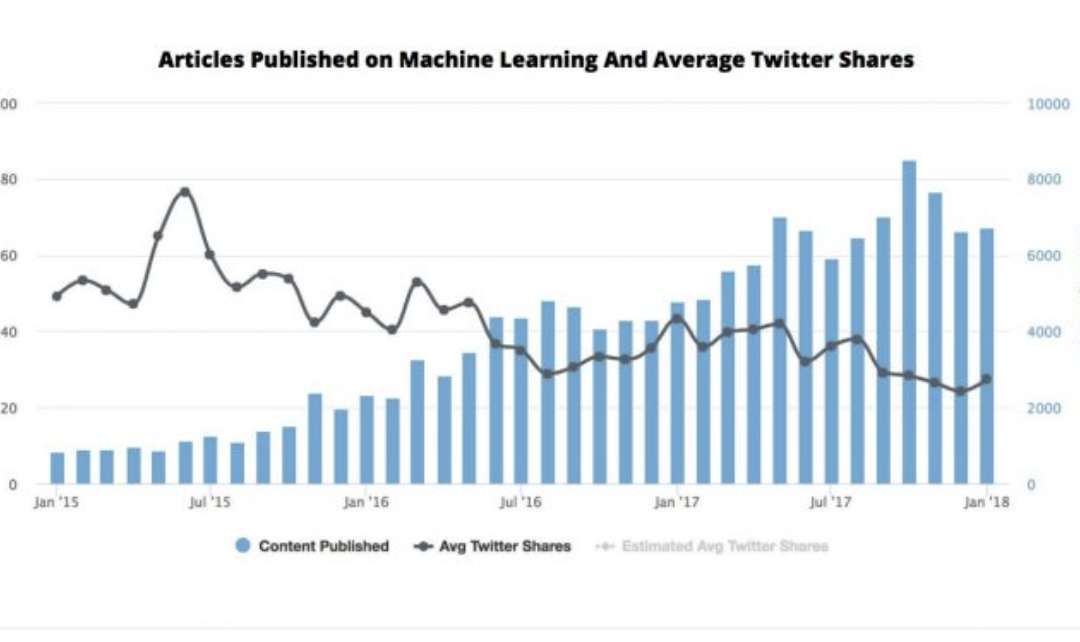
\includegraphics[scale=0.3]{figures/social-share-has-decreased.png}
    \centering
    \caption{Η δημοσιεύσεις κοινωνικών γεγονότων έχουν υποχωρήσει αισθητά. (Πηγή: \cite{[VEN+18]})}
    \label{socialsharing}
\end{figure}


Προκειμένου να επαναπροσδιοριστεί ο ρόλος των εφαρμογών, είναι απαραίτητο να αναθεωρηθούν τα κίνητρα με τα οποία αυτές κεντρίζουν το ενδιαφέρον του χρήστη. Η κοινωνική επίδειξη, να αντικατασταθεί με την κοινωνική συνεισφορά, ενώ η απομόνωση θα πρέπει να δώσει τη θέση της στην επανένταξη του ατόμου στο κοινωνικό σύνολο. Η ενημέρωση μέσω των εφαρμογών, οφείλει να έχει κοινωνικό χαρακτήρα και όχι να προβάλλει την προσωπική ζωή, ή να ωθεί σε κοινωνικά σύνδρομα τους χρήστες \cite{[BBC+18]}. 

\subsection{Ανάγκη της Κοινωνικής Προσφοράς}
Έχοντας υπόψη τα παραπάνω, καταλήγει κανείς εύκολα στο συμπέρασμα ότι υπάρχει μεγάλη ανάγκη να επανασυνδεθεί ο ρόλος των κοινωνικών εφαρμογών με την συνεισφορά για το κοινό συμφέρον. Αν και ζούμε σε μία εποχή όπου η τεχνολογία προχωράει με αλματώδεις ρυθμούς, ελάχιστο είναι το ποσοστό του συνόλου που γνωρίζει για τα επιτεύγματα των συγχρόνων του στους διάφορους επιστημονικόυς τομείς. Ακόμη κι αν το άτομο εκδηλώνει ενδιαφέρον, είναι δύσκολο να ενημερωθεί όταν όλες οι θεματικές περιστρέφονται γύρω από την προσωπική ζωή. Προκύπτει, λοιπόν μια νέα ανάγκη για κινητοποίηση του χρήστη να αλληλεπιδράσει με το κοινωνικό σύνολο. Αυτό είναι εφικτό χρησιμοποιώντας τις δυνατότητες των ήδη γνωστών εφαρμογών, αυτή τη φορά με σκοπό την ενημέρωση για γεγονότα που αφορούν την ευρύτερη πολιτισμική κοινότητα. 

\subsection{Η Έννοια του Πληθοπορισμού}
%Εδώ γράφουμε σύντομα τις τεχνικές/μεθοδολογίες/μοντέλα που πιθανά θα χρησιμοποιήσει η διπλωματική και είναι αναγκαία η κατανόησή τους από τον αναγνώστη πριν από την παρουσίαση της ανάλυσης και σχεδίασης του συστήματος. Πρόκειται για τεχνικές/μεθοδολογίες/μοντέλα που έχουν προταθεί από άλλους και δεν είναι πρωτότυπη δουλειά της διπλωματικής. Μετά βάζουμε μία ενότητα για κάθε τεχνική/μεθοδολογία/μοντέλο, όπου και δίνουμε λεπτομερή περιγραφή.
Συνδυάζοντας τη δύναμη της συλλογικής προσφοράς με την τεχνολογία και τεχνογνωσία που είναι διαθέσιμη σήμερα, η ενημέρωση μπορεί να πάρει νέα διάσταση. Με στοχευμένο προσανατολισμό της κοινωνικής διάθεσης για δράση προς μία συγκεκριμένη κατεύθυνση, η κοινωνία μπορεί να στρατολογήσει τα ίδια τα μέλη της προκειμένου να προάγει τις τεχνολογικές, πολιτισμικές και κοινωνικές εκδηλώσεις, να συντονίσει την πληροφορία και να ενημερώσει το σύνολο. Σύμφωνα με τη \selectlanguage{english}\textit{New York Times}\selectlanguage{greek}, χάρις στην αυξανόμενη συνδεσιμότητα μέσω του διαδικτύου, εκατομμύρια ανθρώπων μπορούν να συνεισφέρουν ιδέες και πληροφορίες για προβλήματα οποιασδήποτε μορφής. Η πρακτική της συμμετοχής ενός «πλήθους» ή μιας ομάδας για έναν κοινο στόχο ή επίλυση κοινών προβλημάτων, με την επιστράτευση της τεχνολογίας ως διαύλου επικοινωνίας ονομάζεται \textit{πληθοπορισμός} (\selectlanguage{english}\textit{Crowdsourcing})\selectlanguage{greek} \cite{[CSW+18]}.

\subsubsection{Εφαρμογές του Πληθοπορισμού}
Τα πεδία στα οποία μπορεί να αξιοποιηθεί η τεχνική του πληθοποριμού είναι αμέτρητα. Ο,τιδήποτε μπορεί να αποκτήσει συνεργατικό χαρακτήρα. Αναφορικά, παρατίθενται μερικοί κλάδοι όπου ανθεί η τεχνική αυτή:
\begin{description}[font=$\bullet$~\normalfont\color{black}]
\item [Εκπαίδευση]
\item [Οικονομία]
\item [Επιστήμη και Υγεία]
\item [ΙΤ]
\item [Διαφήμιση]
\item [Επιχειρηματικότητα]
\item [Κοινωνικές Εκδηλώσεις και ΜΚΟ]
\end{description}

\subsubsection{Μοντέλο Πληθοπορισμού στην Εφαρμογή}
Η εφαρμογή σκοπεύει να χρησιμοποιήσει την πρακτική του πληθοπορισμού για να συγκεντρώσει πληροφορίες σχετικές με πολιτισμικές και κοινωνικές εκδηλώσεις. Οι χρήστες θα έχουν τη δυνατότητα να αξιολογούν τα πάντα γύρω από ένα γεγονός. Θα είναι δυνατή η ενημέρωση για τυχόν αλλαγές της ώρας και του τόπου, για προβλήματα που μπορεί να δυσκολέψουν την διεξαγωγή της εκδήλωσης, ή ιδέες για την καλυτέρευση αυτής. Το σημαντικό στοιχείο όλων των παραπάνω είναι πως θα μπορούν να γίνουν σε πραγματικό χρόνο. Αυτό θα έχει σαν αποτέλεσμα την καλύτερη αλληλεπίδραση μεταξύ συμμετεχόντων και διοργανωτών, την αποφυγή προβλημάτων και παρανοήσεων και την καλύτερη ενημέρωση του πλήθους. Διοργανωτές και συμμετέχοντες, θα μπορούν να εκφράσουν τη γνώμη τους, όλοι ως χρήστες της εφαρμογής. Η πληροφορία θα επικαιροποιείται διαρκώς από όσους παρευρίσκονται ήδη εκεί και θα διαδίδεται σε όσους μέχρι τώρα την αγνοούσαν.Το παραπάνω μοντέλο υλοποιειται μέσω ενός συστήματος μηνυμάτων μεταξύ των χρηστών. 

\section{Σχετικές Ερευνητικές Προσπάθειες και Πρότυπα}
Αν και το παρόν έργο αποτελεί προσωπική πρωτοβουλία, η ιδέα της διπλωματικής έχει κάποιες επιρροές και από άλλα παράλληλα έργα στον ίδιο τομέα. Τέτοια έργα είναι το \selectlanguage{english}\textit{WITHcrowd}\selectlanguage{greek} της ερευνητικής ομάδας του εργαστηρίου Ευφυών Συστημάτων (\selectlanguage{english}\textit{ISLAB}\selectlanguage{greek}) του Εθνικού Μετσόβιου  Πολυτεχνείου, που αποτελεί μέρος του ευρωπαϊκού προγράμματος \selectlanguage{english}\textit{WITH}\selectlanguage{greek}. Το έργο αυτό αποτέλεσε πηγή έμπνευσης για το κομμάτι του πληθοπορισμού στην εφαρμογή της παρούσας εργασίας. Χρησιμοποιήθηκαν επίσης to πρότυπo ανοιχού κώδικα \selectlanguage{english}\textit{Foursquare API}\selectlanguage{greek}, και οι διεπαφές αυτού,  \selectlanguage{english}\textit{Foursquare Autocomplete}\selectlanguage{greek} και \selectlanguage{english}\textit{Foursquare Places}\selectlanguage{greek}. Συνολικά, η εφαρμογή είναι μια καινοτομία η οποία προσπαθεί να στρέψει ήδη υπάρχουσες πρακτικές προς μια νέα κατεύθυνση, χρησιμοποιώντας τις σύγχρονη τεχνογνωσία για έναν πρωτοποριακό σκοπό.   

\subsection{\selectlanguage{english}WITHcrowd}
To \selectlanguage{english}WITHcrowd\cite{[WIT+18]}\selectlanguage{greek} είναι μια πρωτοβουλία της ευρωπαϊκής κοινότητας για τη συλλογή και ταξινόμηση δεδομένων πολιτισμικού περιεχομένου. Αποτελείται από μία πλατφόρμα που εκθέτει τις διεπαφές (ΑΡΙ) διαφόρων πυλών (\selectlanguage{english}portals)\selectlanguage{greek} και ψηφιακών αποθηκών (\selectlanguage{english}repositories)\selectlanguage{greek}. Eπιτρέπει στους χρήστες την αναζήτηση ψηφιακού περιεχομένου από μια σειρά διαφορετικών και ανεξάρτητων αποθετηρίων και βάσεων δεδομένων από ένα ενιαίο σημείο πρόσβασης. Τα αποθετήρια που μπορούν να αναζητηθούν περιλαμβάνουν μεταξύ άλλων την \selectlanguage{english}Europeana,\selectlanguage{greek} την Ψηφιακή Δημόσια Βιβλιοθήκη της Αμερικής, το \selectlanguage{english}YouTube,\selectlanguage{greek} το Μουσείο \selectlanguage{english}Rijks,\selectlanguage{greek} την Εθνική Βιβλιοθήκη της Αυστραλίας και την Ψηφιακή Νέα Ζηλανδία. Όλη η δύναμη της πλατφόρμας συγκεντρώνεται στο γεγονός ότι ο χρήστης είναι υπεύθυνος για την επίτευξη του στόχου του προγράμματος. Αυτή την πρακτική επιχειρεί να υιοθετήσει η εφαρμογή που θα αναλυθεί στα επόμενα κεφάλαια. 

\subsection{\selectlanguage{english}Foursquare API}
Το \selectlanguage{english}\textit{Foursquare API}\cite{[4SQ+18]}\selectlanguage{greek} είναι η διεπαφή της εφαρμογής \selectlanguage{english}\textit{Foursquare}\selectlanguage{greek} και παρέχεται στην κοινότητα της πληροφορικής δωρεάν. Δίνει τη δυνατότητα στους προγραμματιστές να χρησιμοποιήσουν δεδομένα που αφορούν τελικά σημεία (\selectlanguage{english}endpoints)\selectlanguage{greek} σε Ενιαίους Εντοπιστές Πόρων (\selectlanguage{english}URLs)\selectlanguage{greek}, όπως τα στοιχεία μιας υπηρεσίας (πχ. τοποθεσία, πληροφορίες επικοινωνίας, διεύθυνση, όνομα, κατηγορία, ώρες λειτουργίας, παροχές κλπ).

To \selectlanguage{english}\textit{Foursquare}\selectlanguage{greek} έφερε την επανάσταση στα μέσα κοινωνικής δικτύωσης με την καινοτομία του ``\textit{\selectlanguage{english}check in}''.  Η λειτουργία της εφαρμογής \selectlanguage{english}Foursquare\selectlanguage{greek} συνοψίζεται στην αξιολόγηση και άσκηση κριτικής σε κέντρα διασκέδασης, εστιατόρια και χώρους ψυχαγωγίας. Ο χρήστης δημοσιεύει την τοποθεσία του κάνοντας \selectlanguage{english}check in\selectlanguage{greek} και ενημερώνει τους υπόλοιπους χρήστες-φίλους του. Η εφαρμογή που θα υλοποιηθεί κάνει μια απόπειρα να διοχετεύσει την πληροφορία σε αντίστοιχα μέρη πολιτισμικού ή κοινωνικού περιεχομένου και να την αξιοποιήσει για την αξιολόγησή τους.


\section{\selectlanguage{greek}Τεχνολογικό υπόβαθρο - Βασικές Έννοιες}
Στη συνέχεια θα γίνει μια εισαγωγή στις τεχνολογίες και τα εργαλεία προγραμματισμού. Έπειτα ακολουθεί η ανάλυση των σύγχρονων τεχνολογικών μέσων που αποτελούν τη βάση των μεθόδων και μοντέλων που χρησιμοποιήθηκαν στην υλοποίηση της εφαρμογής. 

Όταν ένας προγραμματιστής αναπτύσσει μία εφαρμογή, καλείται να προσδιορίσει τρία πράγματα:
\begin{enumerate}
\item Tην φύση της εφαρμογής - αν θα τρέχει σε φυλλομετρητή (\selectlanguage{english}Web Application)\selectlanguage{greek} ή αν θα είναι μητρική (\selectlanguage{english}Native Application)\selectlanguage{greek}.
\item Την γλώσσα στην οποία θα αναπτύξει την εφαρμογή (\selectlanguage{english}Programming Language)\selectlanguage{greek}
\item Την πλατφόρμα λογισμικού στην οποία θα υλοποιήσει την εφαρμογή (\selectlanguage{english}\textit{SDK})\selectlanguage{greek}
\end{enumerate}

\subsection{Είδη Γλωσσών Προγραμματισμού}
Πρωτού μιλήσουμε για τα είδη των σύγχρονων εφαρμογών, είναι απαραίτητο να αναλύσουμε τις κατηγορίες των αντίστοιχων γλωσσών και τις διακρίσεις μεταξύ αυτών. Μια γλώσσα μπορεί να ανήκει σε μία από τις παρακάτω κατηγορίες:
\begin{description}[font=$\bullet$~\normalfont\color{black}]
\item [Μετταγλωτισμένες ή Μητρικές γλώσσες (\selectlanguage{english}Compiled or Native Languages)]\selectlanguage{greek}
\item [Διαχειριζόμενες Γλώσσες (\selectlanguage{english}Managed Languages)]\selectlanguage{greek}
\item [Δυναμικές Γλώσσες (\selectlanguage{english}Dynamic Languages)]\selectlanguage{greek}
\end{description}Η μητρική γλώσσα (\selectlanguage{english}native language)\selectlanguage{greek} είναι μια γλώσσα που μπορεί να τρέξει στην πλατφόρμα του λειτουργικού συστήματος χωρίς να μετατραπεί σε άλλη μορφή κώδικα από τους μεταγλωττιστές (\selectlanguage{english}compilers)\selectlanguage{greek}. Αυτό σημαίνει πως η υλοποίησή της συνοψίζεται κυρίως στη χρήση μεταγλωττιστών (\selectlanguage{english}compilers)\selectlanguage{greek}, οι οποίοι είναι υπεύθυνοι για τη μετατροπή του κώδικα από γλώσσα μηχανής σε πηγαίο κώδικα (πχ. \selectlanguage{english}\textit{C++, C\#, Java, Swift})\selectlanguage{greek}. Η διαχειριζόμενη γλώσσα (\selectlanguage{english}managed language)\selectlanguage{greek} είναι μια γλώσσα που πρέπει να μετατραπεί ή να ερμηνευτεί πριν να εκτελεστεί στην πλατφόρμα (πχ.\selectlanguage{english} \textit{.NET})\selectlanguage{greek}. Σε αυτή την περίπτωση, ο κώδικας θα εκτελεστεί υπό τη διαχείριση μιας εικονικής μηχανής γλώσσας κοινού χρόνου εκτέλεσης ή, όπως είναι γνωστή,\selectlanguage{english} \textit{CLR}\selectlanguage{greek} \cite{[STR+09],[DEV+03]}. Η δυναμική γλώσσα προγραμματισμού (\selectlanguage{english}dynamic language)\selectlanguage{greek} είναι μια κλάση αποτελούμενη από γλώσσες υψηλού επιπέδου (\selectlanguage{english}high-level programming languages)\selectlanguage{greek}, οι οποίες έχουν την ιδιότητα να εκτελούν πολλαπλές εντολές κατά το στάδιο της εκτέλεσης, σε αντίθεση με τις υπόλοιπες γλώσσες που εκτελούν εντολές στο στάδιο μεταγλώττισης  (πχ.\selectlanguage{english} \textit{Python, JavaScript, PHP, Ruby, MATLAB, Elixir})\selectlanguage{greek} \cite{[MIC05], [ADV09]}.

Οι γλώσσες υψηλού επιπέδου, όπως η \selectlanguage{english}Python\selectlanguage{greek} και η \selectlanguage{english}Ruby\selectlanguage{greek}, έχουν αποκτήσει μεγάλη απήχηση τα τελευταία χρόνια. Για πολλούς, αποτελούν τη νέα γεννιά γλωσσών προγραμματισμού. Ωστόσο οι ρίζες τους ανατρέχουν στις αρχές της δεκαετίας του '50, με την γέννηση της \selectlanguage{english}Lisp\selectlanguage{greek} της πρώτης γλώσσας υψηλού επιπέδου. Πλέον, οι δυναμικές γλώσσες συναντόνται τόσο σε πραγματικά διαδικτυακά συστήματα, όσο και σε εφαρμογές που πριν κυριαρχούσαν οι στατικές γλώσσες προγραμματισμού \cite{[ADV09]}.

Εμείς θα επικεντρωθούμε στην πρώτη κατηγορία, των μητρικών ή αλλιώς μεταφρασμένων γλωσσών προγραμματισμού. Το πλεονέκτημα χρήσης μητρικού κώδικα (\selectlanguage{english}native code\selectlanguage{greek}) βρίσκεται στο γεγονός ότι προγράμματα σε τέτοιες γλώσσες είναι γρηγορότερα, χάρις τον μειωμένο χρόνο επιβάρυνσης (\selectlanguage{english}overhead)\selectlanguage{greek} της διαδικασίας μετάφρασης. Αυτό οφείλεται στην ιδιότητά τους να μεταγλωττίζονται κατά το χρόνο μεταγλώττισης και όχι κατά το χρόνο εκτέλεσης, όπως συμβαίνει με άλλα προγράμματα.

Οι γλώσσες χαμηλού επιπέδου (\selectlanguage{english}low-level programming languages)\selectlanguage{greek} είναι δομημένες έτσι ώστε να υφίστανται την τυπική μεταγλώττιση, ειδικά όταν η αποτελεσματικότητα είναι πρωταρχικό μέλημα, έναντι της μεταγλώττισης που υποστηρίζει πολλές πλατφόρμες (\selectlanguage{english}cross-platform)\selectlanguage{greek}. Για αυτές τις γλώσσες, υπάρχουν περισσότερες ένα-προς-ένα αντιστοιχίες ανάμεσα στο προγραμματισμένο κώδικα και τις λειτουργίες υλικού που εκτελούνται σε κώδικα μηχανής, καθιστώντας ευκολότερο για τους προγραμματιστές τον έλεγχο χρήσης της κεντρικής μονάδας επεξεργασίας και μνήμης με λεπτομέρεια. 
Με κάποια προσπάθεια, είναι πάντα δυνατή η σύνταξη μεταγλωττιστών ακόμα και για παραδοσιακά ερμηνευμένες γλώσσες. Για παράδειγμα, η\selectlanguage{english} Common lisp\selectlanguage{greek} μπορεί να μεταγλωττιστεί σε \selectlanguage{english}Java bytecode\selectlanguage{greek} (στη συνέχεια ερμηνεύεται από την εικονική μηχανή\selectlanguage{english} Java\selectlanguage{greek}), σε κώδικα\selectlanguage{english} C\selectlanguage{greek} (στη συνέχεια, μεταγλωττίζεται στον εγγενή κώδικα μηχανής) ή απευθείας σε εγγενή κώδικα. Οι γλώσσες προγραμματισμού που υποστηρίζουν πολλαπλούς στόχους σύνταξης δίνουν μεγαλύτερο έλεγχο στους προγραμματιστές για να επιλέξουν είτε ταχύτητα εκτέλεσης είτε συμβατότητα μεταξύ πλατφόρμων \cite{[SQA+07]}.

\selectlanguage{english}
\begin{lstlisting}[language=Python, caption=\selectlanguage{greek}Παράδειγμα κώδικα σε \selectlanguage{english}Python]
import numpy as np
 
def incmatrix(genl1,genl2):
    m = len(genl1)
    n = len(genl2)
    M = None #to become the incidence matrix
    VT = np.zeros((n*m,1), int)  #dummy variable
 
    #compute the bitwise xor matrix
    M1 = bitxormatrix(genl1)
    M2 = np.triu(bitxormatrix(genl2),1) 
 
    for i in range(m-1):
        for j in range(i+1, m):
            [r,c] = np.where(M2 == M1[i,j])
            for k in range(len(r)):
                VT[(i)*n + r[k]] = 1;
                VT[(i)*n + c[k]] = 1;
                VT[(j)*n + r[k]] = 1;
                VT[(j)*n + c[k]] = 1;
 
                if M is None:
                    M = np.copy(VT)
                else:
                    M = np.concatenate((M, VT), 1)
 
                VT = np.zeros((n*m,1), int)
 
    return M
\end{lstlisting}

\selectlanguage{greek}
\subsection{Μητρικές Γλώσσες Προγραμματισμού (\selectlanguage{english}Native Programming Languages)}
\selectlanguage{greek}
%Μιλάμε για τις δυνατοτητες τους και τα μειονεκτηματα τους (αναφορα σε σχετικα αρθρα, παραθεση δειγματος κωδικα και παραθεση διαγραμματων με την πτωση της χρησης τους)
Έχοντας προσδιορίσει τις κατηγορίες γλωσσών προγραμματισμού, μπορεί κανείς επομένως να αντιληφθεί την ανάγκη των μητρικών ή αλλιώς μεταγλωττισμένων γλωσσών για την ανάπτυξη εφαρμογών σε συγκεκριμένες πλατφόρμες. Αυτές οι γλώσσες είναι κατά κύριο λόγο σχεδιασμένες να τρέχουν σε μια ορισμένη πλατφόρμα για καλύτερη απόδοση και ευκολότερο σχεδιασμό. Τέτοιες γλώσσες που χρησιμοποιούνται σήμερα στις εφαρμογές κινητών συσκευών είναι η \selectlanguage{english}Swift\selectlanguage{greek} και η \selectlanguage{english}Java\selectlanguage{greek}. Η πρώτη χρησιμοποιείται για την υλοποίηση εφαρμογών σε \selectlanguage{english}iOS\selectlanguage{greek} πλατφόρμες, ενώ η δεύτερη για την ανάπτυξη εφαρμογών που τρέχουν σε \selectlanguage{english}Android\selectlanguage{greek} πλατφόρμες.

\subsubsection{\selectlanguage{english}Swift - iOS Development}
\selectlanguage{greek}
Η \selectlanguage{english}\textit{Swift}\selectlanguage{greek} είναι μια μεταγλωττισμένη, γενικού σκοπού, πολυπαραδειγματική γλώσσα προγραμματισμού που έχει αναπτυχθεί από την \selectlanguage{english}\textit{Apple Inc.}\selectlanguage{greek} για τα προϊόντα τις ίδιας εταιρείας (\selectlanguage{english}\textit{iOS, macOS, watchOS, tvOS}\selectlanguage{greek}). Είναι σχεδιασμένη ώστε να δουλεύει με το \textit{\selectlanguage{english}XCode IDE\selectlanguage{greek}} και χρησιμοποιείται από την κοινότητα των \selectlanguage{english}iOS developers\selectlanguage{greek} για ανάπτυξη \selectlanguage{english}iOS\selectlanguage{greek} εφαρμογών, υποστηριζόμενων από τις πλατφόρμες και τα προϊόντα \selectlanguage{english}Apple\selectlanguage{greek} \cite{[SWIFT1+16]}.

Τα πρώτα βήματα για την δημιουργία της \selectlanguage{english}Swift\selectlanguage{greek} ξεκίνησαν υπό την καθοδήγηση του \selectlanguage{english}C.~Lattner\selectlanguage{greek}, εντός της \selectlanguage{english}Apple\selectlanguage{greek}. Με επιρροές από γλώσσες όπως οι \selectlanguage{english}\textit{Objective-C, Rust, Haskell, C\#}\selectlanguage{greek} και αρκετές ακόμη \cite{[SWIFT2+14]}, η \selectlanguage{english}Swift\selectlanguage{greek} ήρθε στο προσκήνιο επίσημα για πρώτη φορά στο Παγκόσμιο Συνέδριο Προγραμματιστών (\selectlanguage{english}WWDC\selectlanguage{greek}) τον Ιούνιο του 2014 \cite{[SWIFT3+14]}. 

Βασικά γνωρίσματα αυτής της γλώσσας είναι η αντικειμενοστρέφεια (\selectlanguage{english}\textit{OO} language\selectlanguage{greek}), και η απλουστευμένες δομές. Η \selectlanguage{english}Swift\selectlanguage{greek} βασίζεται σε θεωρητικές έννοιες των μοντέρνων γλωσσών προγραμματισμού και προσπαθεί να παρουσιάσει μια απλούστερη συντακτική προσέγγιση \cite{[SWIFT4], [SWIFT5]}. 

\selectlanguage{english}
\begin{lstlisting}[language=Swift, caption=\selectlanguage{greek}Παράδειγμα κώδικα σε \selectlanguage{english}Swift]
    import UIKit
    import AVFoundation
    
class ViewController: UIViewController {
    
    @IBOutlet weak var darkBlueBG: UIImageView!
    @IBOutlet weak var powerBtn: UIButton!
    @IBOutlet weak var cloudHolder: UIView!
    @IBOutlet weak var rocket: UIImageView!
    @IBOutlet weak var hustleLbl: UILabel!
    @IBOutlet weak var onLbl: UILabel!
    
    var player: AVAudioPlayer!
    
    override func viewDidLoad() {
        super.viewDidLoad()
        
        let path = Bundle.main.path(forResource: "hustle-on", ofType: "wav")!
        let url = URL(fileURLWithPath: path)
        do {
            player = try AVAudioPlayer(contentsOf: url)
            player.prepareToPlay()
        } catch let error as NSError {
            print(error.description)
        }
    }
    
    @IBAction func powerBtnPressed(_ sender: Any) {
        cloudHolder.isHidden = false
        darkBlueBG.isHidden = true
        powerBtn.isHidden = true
        
        player.play()
        
        UIView.animate(withDuration: 2.3, animations: {
            self.rocket.frame = CGRect(x: 0, y: 140, width: 375, height: 402)
        }) { (finished) in
            self.hustleLbl.isHidden = false
            self.onLbl.isHidden = false
        }
    }
}

\end{lstlisting}


\subsubsection{\selectlanguage{english}Java - Android Development}
\selectlanguage{greek}
Η \selectlanguage{english}\textit{Java}\selectlanguage{greek} είναι γενικού σκοπού, ταυτοχρονισμένη (\selectlanguage{english}concurrent\selectlanguage{greek}), βασισμένη σε κλάσεις (\selectlanguage{english}class-based\selectlanguage{greek}) και αντικειμενοστραφής (\selectlanguage{english}\textit{OO}\selectlanguage{greek}) γλώσσα \cite{[JAVA1]}. Έχει σχεδιαστεί ειδικά για να επιτρέπει όσο το δυνατό μεγαλύτερη ανεξαρτησία στον προγραμματιστή και ευελιξία όσον αφορά τη συγγραφή κώδικα με συνδυασμό πολλών βιβλιοθηκών. Ακολουθεί τη νοοτροπία ``\selectlanguage{english}\textit{WORA}\selectlanguage{greek}'' \cite{[JAVA2]}, με αποτέλεσμα να μπορεί να τρέξει σε όλες τις πλατφόρμες που υποστηρίζουν \selectlanguage{english}Java\selectlanguage{greek} χωρις να χρείαζεται επαναμεταγλώττιση \cite{[JAVA3]}. Από το 2016 η \selectlanguage{english}Java\selectlanguage{greek} έχει ανέλθει σε μία από τις δημοφιλέστερες εν ενεργεία γλώσσες προγραμματισμού \cite{[JAVA4], [JAVA5], [JAVA6]}.

Η \selectlanguage{english}Java\selectlanguage{greek} εμφανίστηκε στο προσκήνιο το 1991, χάρις στον \selectlanguage{english}J. Gosling\selectlanguage{greek} και τους συνεργάτες του. Η πρώτη επίσημη δημοσίευση έγινε το 1996 από την εταιρεία \selectlanguage{english}Sun Microsystems\selectlanguage{greek} \cite{[JAVA8]}. Σύντομα, ενσωματώθηκε στους σημαντικότερους φυλλομετρητές ιστού (\selectlanguage{english}web browsers\selectlanguage{greek}), και σε ιστοσελίδες (\selectlanguage{english}web pages\selectlanguage{greek}), πράγμα που την μετέτρεψε σε ισχυρό προγραμματιστικό εργαλείο. Η \selectlanguage{english}Java\selectlanguage{greek} δέχθηκε αρκετές επιρροές από τη \selectlanguage{english}C++\selectlanguage{greek}, όσον αφορά το συντακτικό κομμάτι. Όντας επίσης μιας αντικειμενοσταφής γλώσσα προγραμματισμού, η \selectlanguage{english}Java\selectlanguage{greek} θεμελιώνεται σε κλάσεις (\selectlanguage{english}classes\selectlanguage{greek}) και κάθε ομάδα δεδομένων αποτελεί ένα ``\textit{αντικείμενο}'' (\selectlanguage{english}\textit{object}\selectlanguage{greek}). Εξαίρεση αποτελούν οι πρωτογενείς τύποι δεδομένων (πχ \selectlanguage{english}\textit{integers, floating points, boolean values}\selectlanguage{greek} κλπ)

To 2005, η \selectlanguage{english}Google\selectlanguage{greek} ανακοίνωσε ένα νέο λειτουργικό σύστημα προοριζόμενο για φορητές συσκευές με το όνομα \selectlanguage{english}Android\selectlanguage{greek}. Πρόκειται για μια παραλλαγή του πυρήνα του λειτουργικού συστήματος \selectlanguage{english}Linux\selectlanguage{greek}, με προσθήκες από κάποιες ακόμη βιβλιοθήκες ανοιχτού λογισμικού. Το λογισμικό \selectlanguage{english}Android\selectlanguage{greek} υποστηρίζεται από συσκευές 3ης γενιάς (\selectlanguage{english}smartphones, tablets\selectlanguage{greek}) καθώς και άλλα προϊόντα της \selectlanguage{english}Google\selectlanguage{greek} (πχ \selectlanguage{english}\textit{Android Auto, Android TV, Wear OS}\selectlanguage{greek} κλπ). οι εφαρμογές που αναπτύσσονται με αυτό το λειτουργικό σύστημα υλοποιούνται με τη χρήση της πλατφόρμας \selectlanguage{english}\textit{Android Studio SDK} \cite{[JAVA9]}\selectlanguage{greek} και της γλώσσας \selectlanguage{english}Java \cite{[JAVA10]}\selectlanguage{greek}. Την πλατφόρμα αυτή συνοδεύουν και άλλα χρήσιμα εργαλεία, όπως αποσφαλματωτής (\selectlanguage{english}debugger\selectlanguage{greek}), βιβλιοθήκες λογισμικού και προσομοιωτής (\selectlanguage{english}emulator\selectlanguage{greek}) \cite{[JAVA11]}.

\selectlanguage{english}
\begin{lstlisting}[language=Java, caption=\selectlanguage{greek}Παράδειγμα κώδικα σε \selectlanguage{english}Java]
// This is an example of a single line comment using two slashes

/* This is an example of a multiple line comment using the slash and asterisk.
 This type of comment can be used to hold a lot of information or deactivate
 code, but it is very important to remember to close the comment. */

package fibsandlies;
import java.util.HashMap;

/**
 * This is an example of a Javadoc comment; Javadoc can compile documentation
 * from this text. Javadoc comments must immediately precede the class, method, or field being documented.
 */
public class FibCalculator extends Fibonacci implements Calculator {

    private static Map<Integer, Integer> memoized = new HashMap<Integer, Integer>();

    /*
     * The main method written as follows is used by the JVM as a starting point for the program.
     */
    public static void main(String[] args) {
        memoized.put(1, 1);
        memoized.put(2, 1);
        System.out.println(fibonacci(12)); //Get the 12th Fibonacci number and print to console
    }

    /**
     * An example of a method written in Java, wrapped in a class.
     * Given a non-negative number FIBINDEX, returns
     * the Nth Fibonacci number, where N equals FIBINDEX.
     * @param fibIndex The index of the Fibonacci number
     * @return The Fibonacci number
     */
    public static int fibonacci(int fibIndex) {
        if (memoized.containsKey(fibIndex)) {
            return memoized.get(fibIndex);
        } else {
            int answer = fibonacci(fibIndex - 1) + fibonacci(fibIndex - 2);
            memoized.put(fibIndex, answer);
            return answer;
        }
    }
}


\end{lstlisting}



\subsection{\selectlanguage{english}JavaScript}
\selectlanguage{greek}
Μιλαμε εισαγωγικα για τη γλωσσα αυτη, ιδεες απο τη διπλωματικη του παιδιου και περναμε στην Ρεακτ. Μιλαμε για τα γνωρισματα και τα πλεονεκτηματα της (παρε την περιληψη που εγραψες).

\subsubsection{\selectlanguage{english}React Native}

